\section{Experiments}
We did five dumps of the memory;
  \subsection{Clean dump}
The first dump we did was right after boot, with factory settings and nothing 
done to the device other than transferring the LiME LKM to the SD-card. The 
reason for this dump so we could see if we had set up our environment correctly 
and could read memory of the phone. The dump was also great for use when 
comparing to later dumps where we could see differences from a system with no 
significant use and compare them to the other experiments. This experiment
thus served more as a control, and we were not looking for any specific data in
memory. We used the experiment to test if we had set up and configured 
Volatility correctly. We were able to run Volatility on the memory dump, an 
verified that we got out sensible data from it, such as process list, and 
process tree. We also tested PhotoRec on the memory dump, and it successfully
extracted whole and partial images, text files, and Java code and class files.
It also managed to find syslog(dmesg), and other log files that could be useful
in a forensic investigation.
  
\subsection{Pastebin entry}
The second dump we did was after creating a pastebin entry on pastebin.com using
the stock Android browser (for 4.2.2), to see if we could find our entry in the 
memory. When starting to analyze this dump, we first started with the most basic.
Strings and hex editor; by searching for \texttt{pastebin.com}. Other findings in
this process included a timeline on how the user got to the page pastebin.com by 
examining the memory segments before the hit on our string.\\

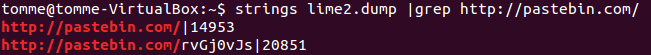
\includegraphics[scale=0.48]{strings_grep_pastebin.png}

%timeline wtf?

Finding the message, and link for the pastebin entry with \texttt{strings} and a
hex editor was not a problem, this was accomplished by a simple string search for
the string \textit{pastebin}. We were also able to find the data using Volatility's
\texttt{yarascan} plugin. The plugin allows searching by using simple strings,
or with more complex rules. For unknown reasons Volatility was not able to find
the list of running processes of this memory dump, and it had to search through 
the whole memory dump for finding the entry instead of reducing the search space 
by specific PID. 
  
\subsection{Standard Text Message}
In the third experiment we sent a text message to the standard messages application.
This was done by using the emulators’ telnet interface, where one can send a message
using the form: \texttt{sms send <phoneNumber> <textMessage>}. After sending the
message, a dump of the memory was taken. We wanted to see if it was possible to 
see recently received messages from the memory dump. Since we already knew the 
contents of the message, it was a simple matter of locating it in the memory 
dump using previous mentioned tools to do a text search. In the output of the
\texttt{yarascan} plugin we could also see the time, and phone number that was
used to send the message.
  
\subsection{Secure application - TextSecure}
Next we repeated the same experiment as above, but using the TextSecure
\footnote{\url{https://play.google.com/store/apps/details?id=org.thoughtcrime.securesms}}, 
messaging application, which encrypts messages on the disk and over the wire.
TextSecure was chosen since it is a commonly used application for securing your 
text messages in transit (both sender and receiver would need to have it 
installed) and it is open source so we could get a better understanding on 
how it manages the keys and data in memory.  
In some cases the device might have used anti-forensic tools to hide their 
activity, we wanted to look into what information a memory analysis could 
retrieve. In this experiment we were not able to retrieve any data of the message 
data.
\begin{wrapfigure}{r}{0.5\textwidth}
    \begin{center}
        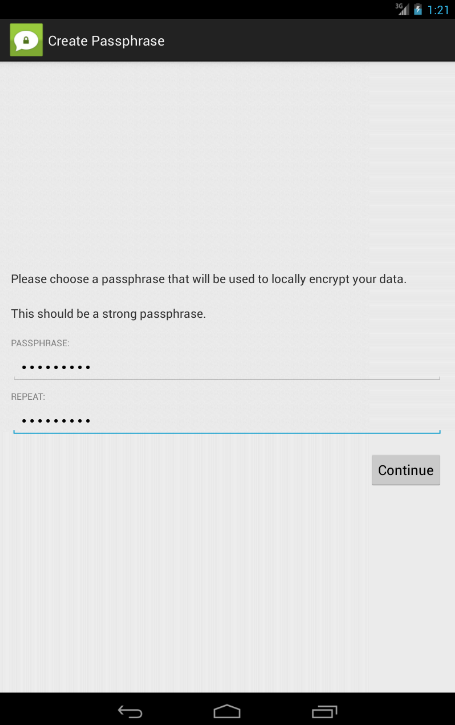
\includegraphics[scale=0.40]{textsecure.png}
    \end{center}
\end{wrapfigure}

\subsection{Screen lock}
We also did a memory dump after creating a screen lock with a PIN code and using a passphrase.
  \paragraph{Strings}
  Strings would show a lot of results since there are often many hits on readable 
  data in these kind of dumps, by piping the output to grep we were able to 
  filter out text we wanted. Simply searching for pastebin.com we were able to 
  find the page it was posted on. We also found the exact message posted to pastebin with strings.
  %Fant vi teksten som var skrevet også? brukte vi vol til dette? (yarascan) => Ja. Fant den også med strings/hex

There is also a Volatility plugin created to get the PIN or passphrase from the
memory dump (\texttt{dalvik\_password}),  %??
But we had no success using this plugin.

If the device has a unlocked bootloader it would often be possible to use our 
method to retrieve memory of a device without wiping off all data from the 
device. This experiment was done to see if we could find a passphrase or 
pincode from the memory dump. By searching for the pincode and passphrase we saw a pattern \\


\begin{figure}
        
        \begin{subfigure}[b]{0.3\textwidth}
                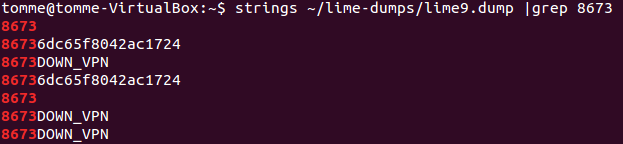
\includegraphics[scale=0.48]{strings_grep_pin.png}
                \caption{Image showing the output of strings piped into grep
                which is looking for the pin.}
                \label{fig:gull}
        \end{subfigure}%
        \qquad \qquad \qquad \qquad \qquad %add desired spacing between images, e. g. ~, \quad, \qquad, \hfill etc.
          %(or a blank line to force the subfigure onto a new line)
        \begin{subfigure}[b]{0.3\textwidth}
                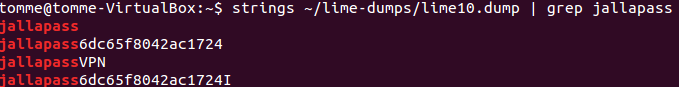
\includegraphics[scale=0.48]{strings_grep_pass.png}
                \caption{This image shows the same, but searching for a
                password instead, notice what seems to be half of a hash appended
            to the password and pin in both images.}
                \label{fig:tiger}
        \end{subfigure}
        \vspace{-20pt}

\end{figure}

